\documentclass[crop]{standalone}
\usepackage{amssymb}
\usepackage{amsmath}
\usepackage{amsfonts}
\usepackage{color}
\usepackage{tikz}
\usetikzlibrary{math}
\usepackage{tkz-euclide}

\begin{document}
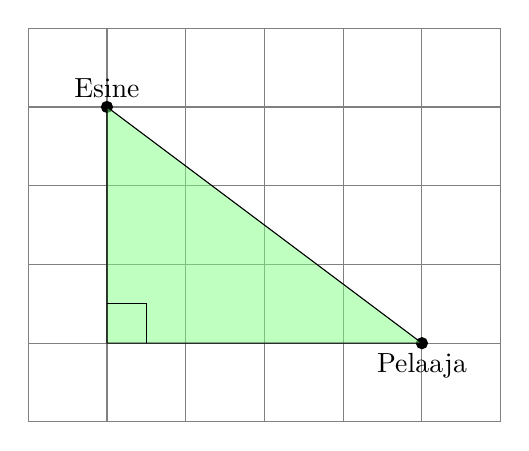
\begin{tikzpicture}
   \tkzInit[xmax=5,ymax=4,xmin=-1,ymin=-1]
   \tkzGrid
   %\tkzAxeXY
   \coordinate (P) at (4,0);
   \coordinate (E) at (0,3);
   \draw[fill=black] (P) circle (2pt) node[below] {Pelaaja};
   \draw[fill=black] (E) circle (2pt) node[above] {Esine};
   \draw[fill=green!50,fill opacity=0.5] (P) -- (0,0)--(E)--(P);
   \draw (0,0.5)-|(0.5,0);
  \end{tikzpicture}
\end{document}